% preamble and style file for M&R lecture slides
\documentclass[11.5pt,sans,english]{beamer}

\usetheme{EastLansing}
\usecolortheme{lily}

\usepackage[most]{tcolorbox}

\usepackage{verbatim}
%\usepackage{ulem}
%\usepackage{fontawesome}
%\usepackage{tikz}
%\usepackage{pifont}
%\usepackage{tabularx}
\usepackage{array,booktabs,xcolor,colortbl,multirow,rotating,amssymb}
%\usepackage{amsmath}
% \usepackage{vwcol}
% \usepackage[T1]{fontenc}

  
\newcommand\vect[1]{\underline{\mathbf{#1}}}
\newcommand\unitvect[1]{\hat{\boldsymbol{#1}}}
%\newcommand\hatdot[1] { \hat{ \dot{ \boldsymbol{#1} } } }

\newtcbox
{\keyc}{on line,arc=2pt, colback=yellow!30!white, colframe=yellow!30!black, before upper={\rule[-3pt]{0pt}{10pt} },boxrule=1pt,boxsep=0pt,left=6pt,right=6pt,top=2pt,bottom=2pt,}

\newtcbox
{\keyb}{on line,arc=1pt, colback=blue!30!white, colframe=blue!30!black, before upper={\rule[-3pt]{0pt}{10pt} },boxrule=1pt,boxsep=0pt,left=6pt,right=6pt,top=2pt,bottom=2pt,}

\newtcbox
{\keyl}{on line,arc=1pt, colback=pink!30!white, colframe=blue!30!black, before upper={\rule[-3pt]{0pt}{10pt} },boxrule=1pt,boxsep=0pt,left=6pt,right=6pt,top=2pt,bottom=2pt,}

\newtcbox
{\keyw}{on line,arc=1pt, colback=red!30!white, colframe=blue!30!black, before upper={\rule[-3pt]{0pt}{10pt} },boxrule=1pt,boxsep=0pt,left=6pt,right=6pt,top=2pt,bottom=2pt,}

\newtcbox
{\keya}{on line,arc=1pt, colback=purple!30!white, colframe=blue!30!black, before upper={\rule[-3pt]{0pt}{10pt} },boxrule=1pt,boxsep=0pt,left=6pt,right=6pt,top=2pt,bottom=2pt,}

\newtcbox[auto counter,number within=section]
{keyf}
{
enhanced,
on line,
  boxsep=0pt,
  left=6pt,right=6pt,top=2pt,bottom=2pt,
  arc=5pt,
  boxrule=1pt,
  rightrule=38pt,
colback=green!10!white, 
colframe=green!50!black, 
title=\thetcbcounter,
detach title,
overlay unbroken and first ={
    \node[%rotate=90,
          %minimum width=1cm,
          anchor=south,
          font=\sffamily\bfseries\tiny,
          %yshift=-10pt,
          yshift=-5pt,
          xshift=-20pt,
          white]
    at (frame.east) {\thetcbcounter};
  }
}


\usepackage{xcolor}

%\usepackage{hyperref}
%\hypersetup{
%  pdfauthor={Lily Asquith},
%  urlcolor=blue,
%  colorlinks=true,
%  linkcolor=blue,
%  bookmarks=true
%}

%---------------------------------------------%
%              LILY'S COLOURS           %
%---------------------------------------------%
\definecolor{Wash}{RGB}{204,204,204}
%\definecolor{Pinky}{RGB}{254,200,254}%violet
\definecolor{Pinky}{RGB}{219,	240,	253}%violet
\definecolor{Bluey}{RGB}{0,190,255}%deep sky blue
\definecolor{DarkGrey}{RGB}{28,66,137}%dar grey
\definecolor{SussexWhite}{RGB}{253,255,254}%dar grey
\definecolor{LightGray}{RGB}{184,184,255}
\definecolor{YesGreen}{RGB}{0,128,0}
\definecolor{NoRed}{RGB}{250,0,0}



\definecolor{myred}{RGB}{255,153,153}
\definecolor{myorange}{RGB}{255,204,153}
\definecolor{myyellow}{RGB}{255,255,153}
\definecolor{mygreen}{RGB}{153,255,153}
\definecolor{mycyan}{RGB}{153,255,255}
\definecolor{myblue}{RGB}{153,204,255}
\definecolor{myviolet}{RGB}{153,153,255}
\definecolor{mypurple}{RGB}{204,153,255}
\definecolor{mypink}{RGB}{255,204,255}
\definecolor{mycoral}{RGB}{255,153,204}

%-----------------------------------------------------%
%              LILY'S COLUMN TYPES          %
%-----------------------------------------------------%
\newcolumntype{a}{>{\raggedright\arraybackslash}l}	
\newcolumntype{q}{>{\raggedright\arraybackslash}m{8cm}} 

%--------------------------------------------%
%              LILY'S SYMBOLS          %
%--------------------------------------------%
\newcommand{\dfinger}{\large{\textcolor{black}{\ding{43}}}\scriptsize}
\newcommand{\dstar}{\large{\textcolor{black}{\ding{76}}}\scriptsize}
\newcommand{\dwrite}{\large{\textcolor{black}{\ding{45}}}\scriptsize}
\newcommand{\ddiamond}{\small{\textcolor{DarkGrey}{\ding{117}}}\scriptsize}
\newcommand{\ddiamondwhite}{\small{\textcolor{SussexWhite}{\ding{117}}}\scriptsize}
\newcommand{\experiment}{\small{\textcolor{magenta}{\faCogs }}\scriptsize}
\newcommand{\watchit}{\textcolor{blue}{ \faYoutube}}


\makeatletter
\newcommand\notsotiny{\@setfontsize\notsotiny{6.5}{7.5}}
\makeatother


% 
\title[ Intro to Quantum Physics]{Intro to Quantum Physics F3241}
%\subtitle{\textbf{Part 2: The Electron}}
\author[Dr Lily Asquith (Lily)]{ Dr Lily Asquith (Lily)}
\date[04 - 08 Oct 2021]{ 04 - 08 Oct 2021 (Week 2)}
\logo{

\includegraphics[width=1.5cm]{../../utils/uslogo.jpg}
}


\begin{document}


\begin{frame}
\titlepage
\end{frame} 

 %-----------------------------------------------------------%
 % 1 Kinematics                                                 %
 %-----------------------------------------------------------%
\section{I2Q Part 2: The Electron}

 
 %-----------------------------------------------------------%
 % LECTURE 1
 %-----------------------------------------------------------%
 



\begin{frame}{This Week: The Electron}
\small
We have two lectures a week (Monday \& Thursday - your calendars should reflect this now.)\\[1ex]
\begin{itemize}
\item Understanding electricity
\item The discovery of the electron
\end{itemize}
\end{frame}




 \subsection{The Electrical Force and Faraday's Electrolysis}

%  
\begin{frame}{The Electrical Force}
\small
Electric fish: Thunderers of the Nile,  protectors of all other fish.\\[1ex]

\begin{center}
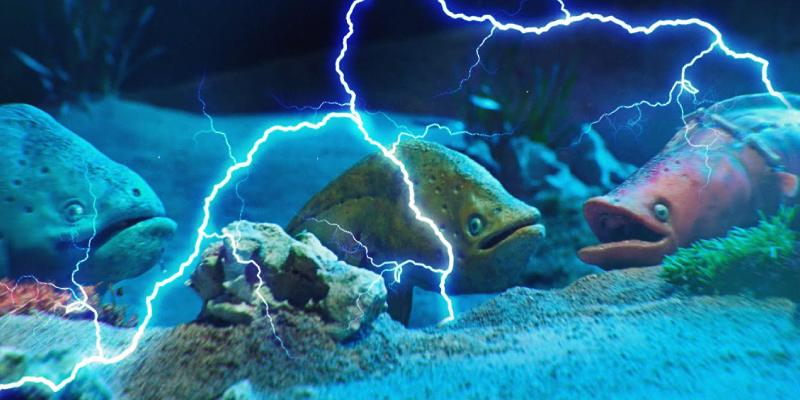
\includegraphics[scale=0.3]{fish.jpg}
\end{center}
\end{frame}


\begin{frame}{Triboelectricity (\textit{tribo: rubbing})}
\small
\begin{itemize}
\item Evidence suggests first \textbf{ use} of electricity was amber spindles, used in weaving.
\item Amber attracts feathers when rubbed, glass repels them: 'Resinous' and 'Vitreous'.
\item Amber, resin, rubber, polystyrene : positively charged
\item Glass, skin, fur, silk : negatively charged
\end{itemize}
\begin{center}
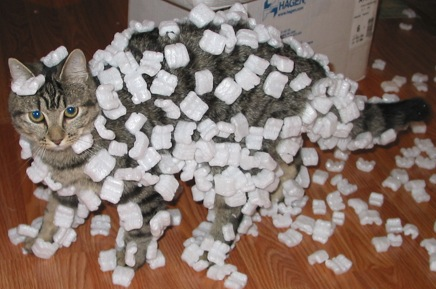
\includegraphics[scale=1]{cat.jpg}
\end{center}
\tiny
Sean McGrath,  CC BY 2.0 

\small
We now know that this force comes from the exchange of electrons between the materials.
\end{frame}


\begin{frame}{Electrical Effluvia }
\small
\begin{itemize}
\item Gilbert 1600 hypothesized that the amber effect could be explained by an effluvium (a small stream of particles that flows from the electric object, without diminishing its bulk or weight) that acts on other objects
\item Gray 1729 noticed that a cork placed in a glass tube took on its charge. Also wires  across hundreds of metres. Also showed that you don't need objects to touch.\\
\item Were there two kinds of effluvium? This was a popular idea, to explain the attraction or repulson depending on the materials\\
\item Franklin 1750 : actually we only need one fluid. A rubbed glass received the same, but opposite, charge strength as the cloth used to rub the glass\\

\end{itemize}


\end{frame}



\begin{frame}{Investigating electricity}
\small
Charles-Augustin de Coulomb was first (1785) to publish: electrostatic force follows an inverse square law.\\[2ex]

Coulomb's Law: $F = k \frac{q_1 q_2}{r^2}$\\[2ex]

\begin{center}
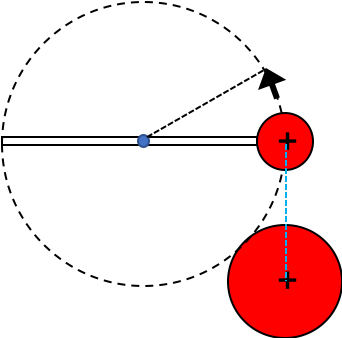
\includegraphics[scale=0.5]{torsion}
\end{center}




%\includegraphics[scale=0.2]{faraday.jpg}

\end{frame}



\begin{frame}{A new era }
\small

Volta 1800: came up with a way to store charge, providing continuous current. %Also, $Q=CV$


\begin{center}
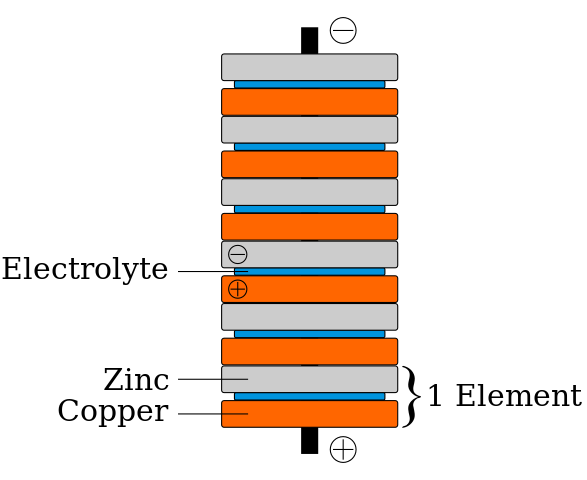
\includegraphics[scale=0.3]{voltaic-pile}
\end{center}
\tiny
 Luigi Chiesa, CC BY-SA 3.0 
\end{frame}




\begin{frame}{Investigating electricity}
\small
Michael Faraday devised an \textit{inspired} experiment (1833) to investigate electricity.\\

%\begin{center}

%\includegraphics[scale=0.2]{faraday.jpg}
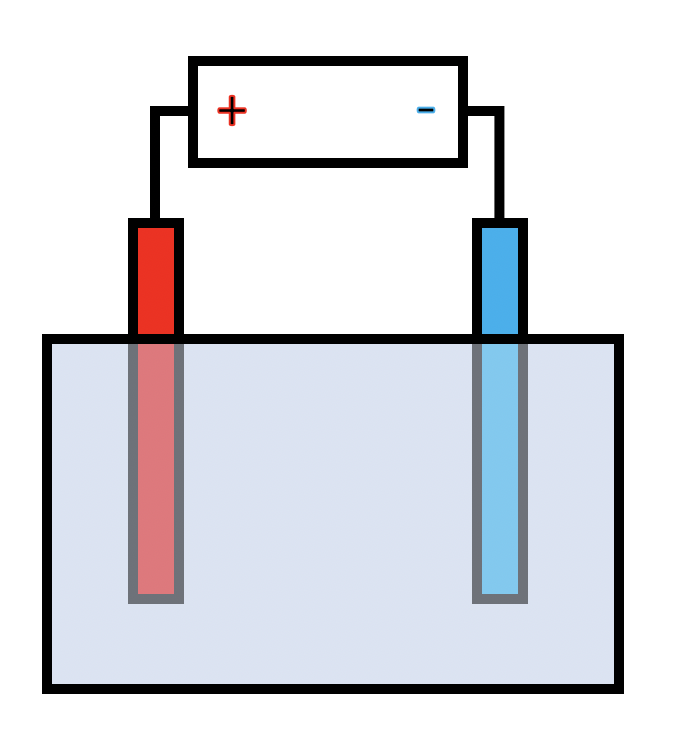
\includegraphics[scale=0.4]{electrolysis}
%\end{center}
\end{frame}


\begin{frame}{Two massive things}
\small
\vspace{2cm}
\begin{enumerate}
\item All substances have something fundamental in common, and this is encoded in $N_A$
\item The behaviour of all substances is described using a common parameter: the fundamental unit of charge $e$
\end{enumerate}
\vspace{2cm}

\tiny
Reminder: $N_A $ is the number of atoms with $Z=n$ in $n$ grams of a substance made of those atoms. \\
Note for H, $Z=1$, so there are $N_A$ atoms in 1 gram of H.
\end{frame}

\begin{frame}{Another massive thing}
\small
Why are these people all of a particular type?\\[1ex]
%Homo Sapiens Sapiens evolved to be the dominant species on this planet under very harsh conditions ()\\[1ex]
Once dominance is achieved, often by terrible means or just by pure luck, no type of human is expected to give that privilege up...\\[1ex]
... but, vast amounts of evidence that all parts of society, including science, benefit from diversity in background and in opinion\\[1ex]
Let us remember that if Newton had been female, he would probably have been burned as a witch.\\[1ex]
Let us also remember that most of the history of science is completely unknown to us: we just have the part that is written.\\[2ex]

\tiny
Yuval Noah Harari:  Sapiens
\end{frame}

\begin{frame}{Further investigations}
\small
Thomson's experiments with a `cathode ray tube', 1897\\[1ex]
Millikan's experiments with an `oil drop' 1909\\[1ex]

Both of these experiments relied on \textbf{equating forces}:\\[1ex]

The Lorentz force (1895) $F = q\vect{E} +q (\vect{v} \times \vect{B})$  links the forces arising from electric and magnetic fields (E and B)\\[1ex]

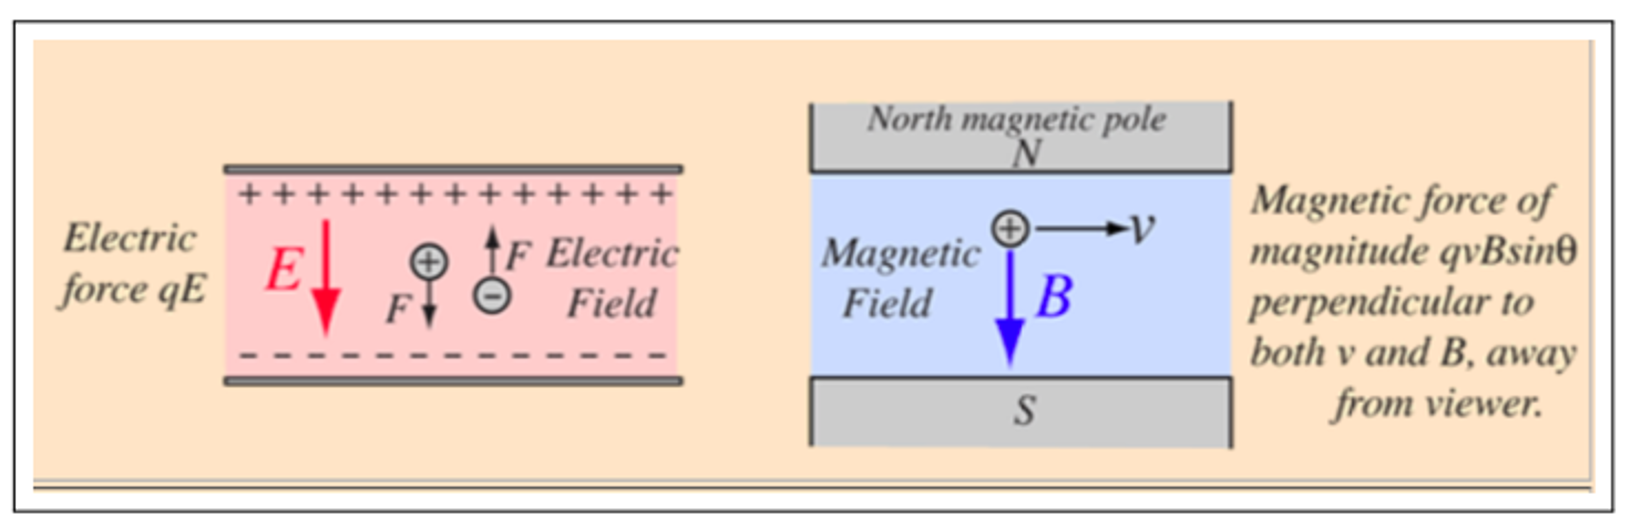
\includegraphics[scale=0.3]{lorentz}
%The centripetal force (1659-89)  $F = \frac{mv^2}{r}$\\
%Newton's Law: $F = k \frac{m_1 m_2 }{r^2}$ \\
%Coulomb's Law: $F = k \frac{q_1 q_2}{r^2}$\\
\end{frame}


\begin{frame}{The electric and magnetic forces}
\small

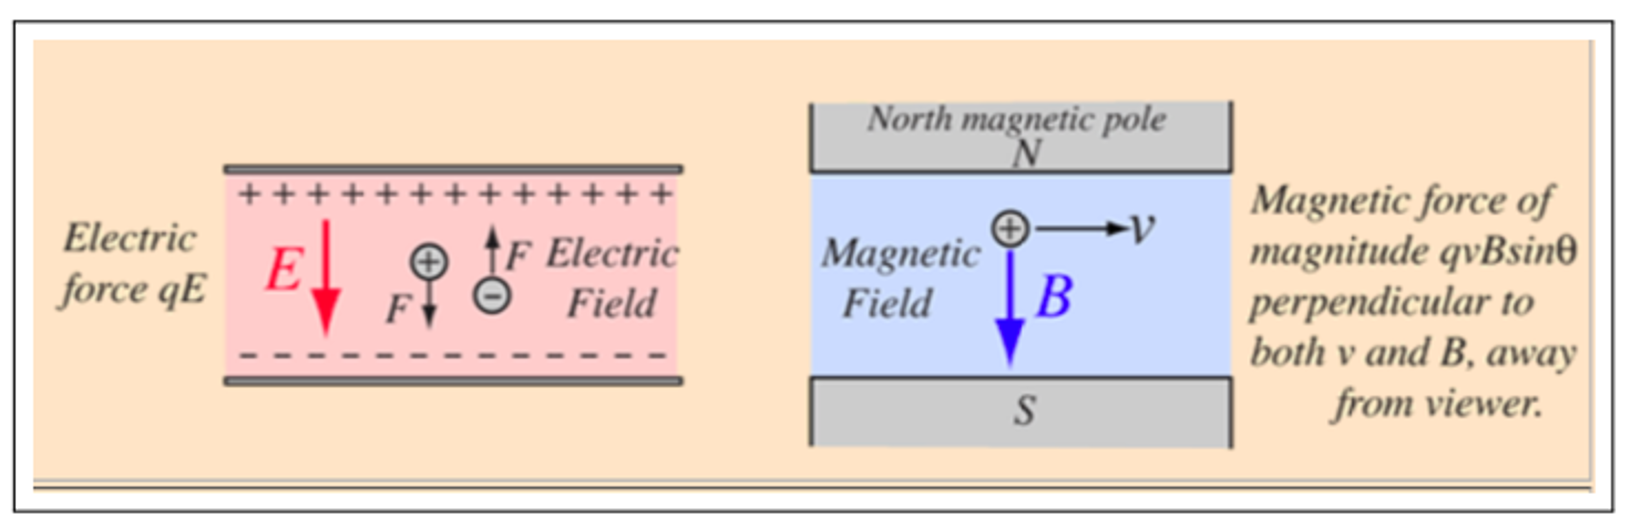
\includegraphics[scale=0.4]{lorentz}
\vspace{5cm}
%The centripetal force (1659-89)  $F = \frac{mv^2}{r}$\\
%Newton's Law: $F = k \frac{m_1 m_2 }{r^2}$ \\
%Coulomb's Law: $F = k \frac{q_1 q_2}{r^2}$\\
\end{frame}



\begin{frame}{Further investigations}
\small

The Lorentz force $F = q\vect{E} +q (\vect{v} \times \vect{B})$ is very useful for understanding the properties of charged particles.\\[2ex]
A trick we can use for things moving in circular motion is $\vect{F} = \frac{mv^2}{r}$. \\[2ex]
It is based on the observation that all circular motion has a related force (gravity, tension, contact, etc)\\[2ex]
\vspace{3cm}
Another trick we can use, for things near Earth's surface, is $F = mg$\\[1ex]
%Newton's Law: $F = k \frac{m_1 m_2 }{r^2}$ \\
%Coulomb's Law: $F = k \frac{q_1 q_2}{r^2}$\\
\end{frame}

\begin{frame}{An example problem - part 1}
\small
We accelerate a mixed beam of electrons and protons to $3 \times 10^7$ ms$^{-1}$, and allow them to enter a region with a uniform magnetic field perpendicular to their direction with a strength of 8T. What happens to the particles?\\[21ex]

%I will use $F=qvB$, so dimensionally $MLT^{-2} = IT LT^{-1}$ [x unknown Tesla dimension]\\
%%unknown Tesla dimension  = $MLT^{-2} I^{-1}T^{-1} L^{-1}T$ \\
%unknown Tesla dimension  = $MT^{-2} I^{-1}$ \\[1ex]
%Units $T = kg s^{-2} A^{-1} = kg s^{-1} C^{-1}$\\[1ex]
%
%
%
%mass of electron = $9.11 \times 10^{-31}$ kg\\[1ex]
%mass of proton = damn it can't remember, but i do remember it is about 2000 times the mass of the electron \\[1ex]
\end{frame}

\begin{frame}{An example problem - part 2}
\small
We accelerate a mixed beam of electrons and protons to $3 \times 10^7$ ms$^{-1}$, and allow them to enter a region with a uniform magnetic field perpendicular to their direction with a strength of 8T. What happens to the particles?\\[21ex]

%I will use $F=qvB$, so dimensionally $MLT^{-2} = IT LT^{-1}$ [x unknown Tesla dimension]\\
%%unknown Tesla dimension  = $MLT^{-2} I^{-1}T^{-1} L^{-1}T$ \\
%unknown Tesla dimension  = $MT^{-2} I^{-1}$ \\[1ex]
%Units $T = kg s^{-2} A^{-1} = kg s^{-1} C^{-1}$\\[1ex]
%
%
%
%mass of electron = $9.11 \times 10^{-31}$ kg\\[1ex]
%mass of proton = damn it can't remember, but i do remember it is about 2000 times the mass of the electron \\[1ex]
\end{frame}


\begin{frame}{Next Lecture}
\small
See you all Thursday when we will think about the Thomson and Millikan experiments.
\end{frame}


%-----------------------------------------------------
%     LECTURE 2
%-----------------------------------------------------
%
%\subsection{Thomson's Experiment: Bendy Rays}
%
%
%
%
%\begin{frame}{}
%\small
%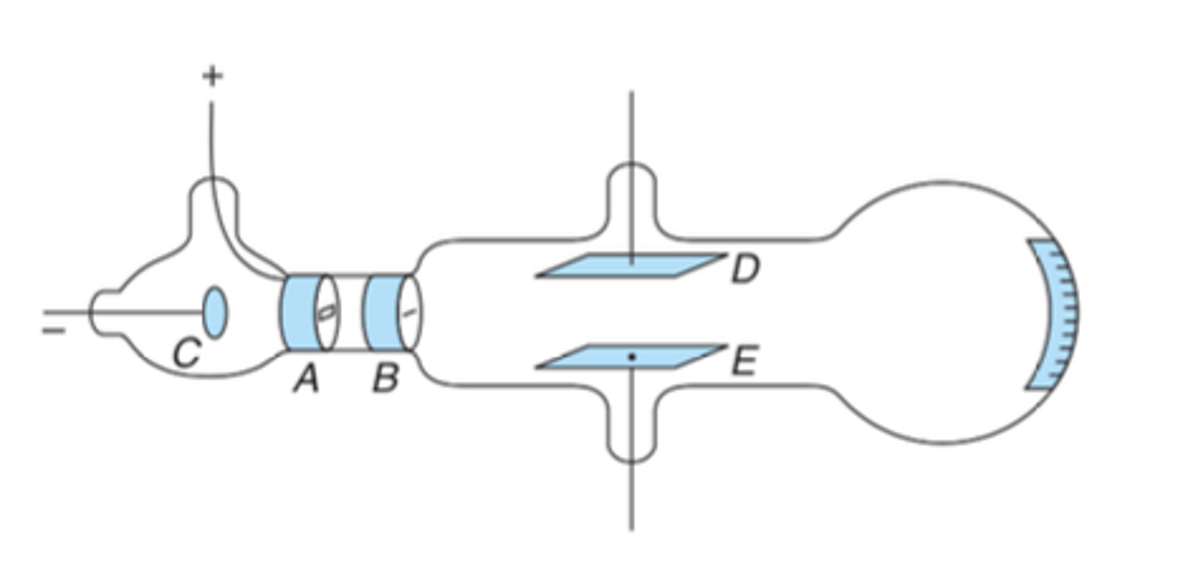
\includegraphics[scale=0.4]{cathode1}
%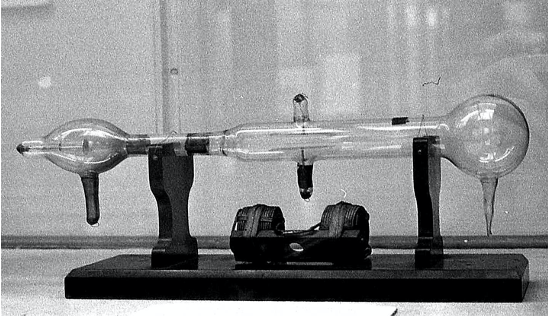
\includegraphics[scale=0.4]{cathode2}
%\end{frame}
%
%
%
%\begin{frame}{}
%\small
%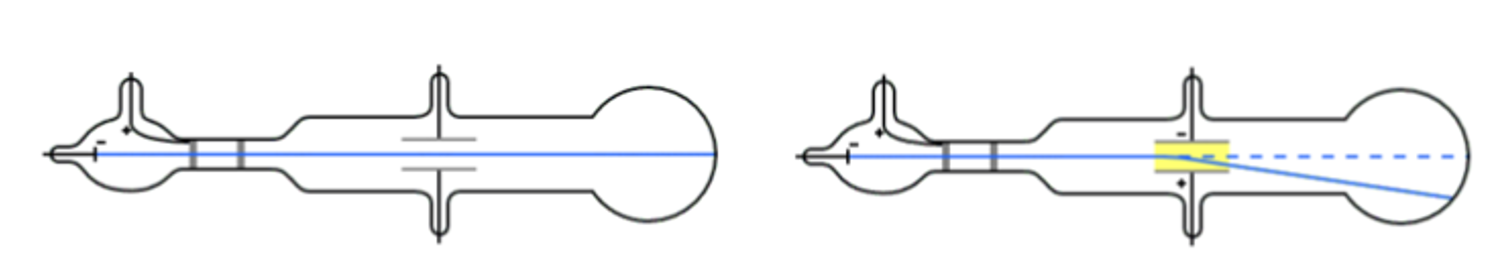
\includegraphics[scale=0.4]{cathode3}
%\end{frame}
%
%
%\begin{frame}{An example problem}
%\small
%
%\end{frame}
%
%%-----------------------------------------------------
%%     LECTURE 3
%%-----------------------------------------------------
%
%\subsection{Millikan's Experiment: Balancing forces}
%
%
%\begin{frame}{}
%\small
%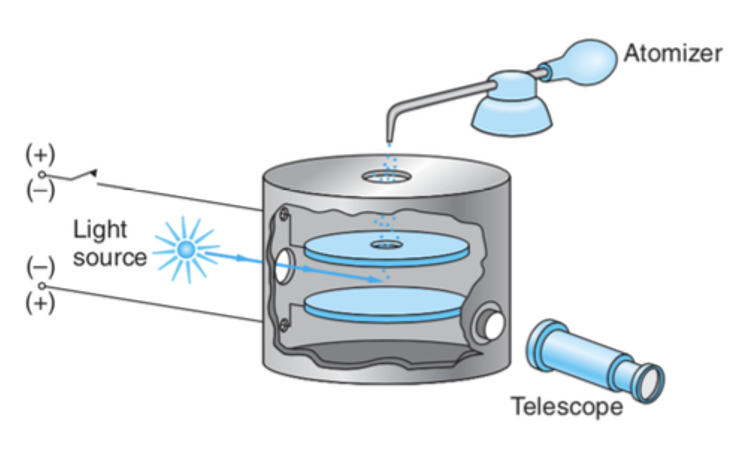
\includegraphics[scale=0.4]{millikan1}
%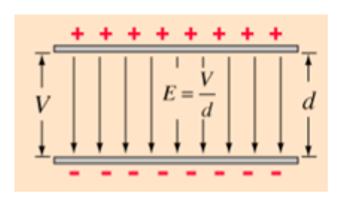
\includegraphics[scale=0.4]{millikan2}
%\end{frame}
%
%
%
%\begin{frame}{An example problem}
%\small
%
%\end{frame}
%
%\begin{frame}{A summary of these two great experiments}
%\small
%Thomson balanced the magnetic and electric forces to get a value for the ratio $\frac{e}{m_e}$\\[2ex]
%Millikan balanced the gravitational and electric forces to get a value for  $m_e$\\[2ex]
%\end{frame}


 
\end{document}